\maketitle
\begin{frame}
    \frametitle{Inhalt}
    \tableofcontents
\end{frame}

\begin{frame}
    \frametitle{Was ist Style Transfer}

    \begin{figure}[H]
        \centering
        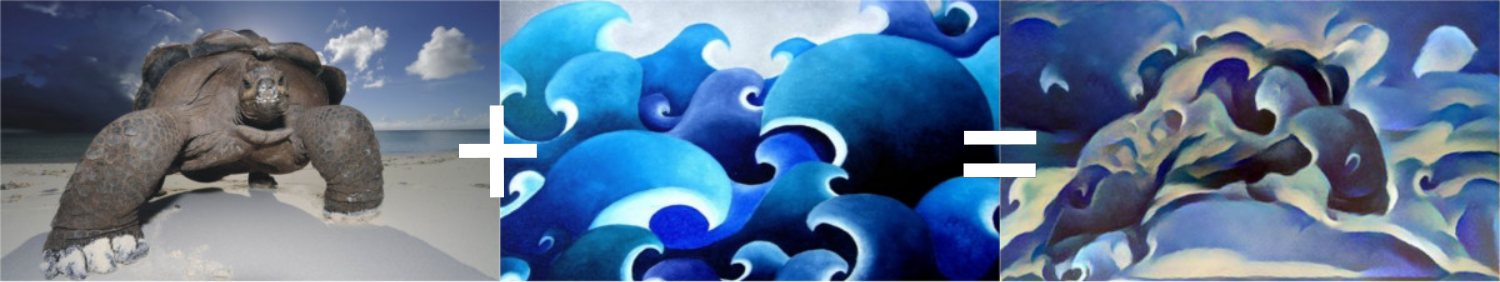
\includegraphics[width=1.0\textwidth]{resources/neuralstyle.png}
        \caption{Kombination von Stil und Inhalt \cite{pytorch_turtle_img}}
        \label{img:pytorch_turtle_img}
    \end{figure}
\end{frame}